\chapter{Gestión, metodología y planificación}\label{cap:gestion}\label{cap:metodologia}

Este capítulo describe cómo se gobernó el trabajo de principio a fin y por qué esa forma de
gobernarlo es, en sí misma, una aportación del TFG y no solo un procedimiento administrativo.
La mayor parte de los proyectos de software describen su metodología en un párrafo y pasan
enseguida al producto. Aquí se dedica un capítulo completo porque el propio proceso de
ingeniería, gobernado de forma sistemática mediante GSD, se trató con
la misma exigencia de evidencia, trazabilidad y verificación que cualquier otra parte del
sistema.

El capítulo fija primero los objetivos de gestión y el método de trabajo, describe después la
planificación viva, la trazabilidad y los agentes que instrumentan ese método, recoge la
planificación del laboratorio de evaluación, la planificación temporal, el esfuerzo y el
presupuesto; termina con los riesgos, las lecciones aprendidas y una valoración de la
metodología.

\section{Objetivos de gestión y método de trabajo}\label{sec:met-objetivos-gestion}\label{sec:gestion-problema}\label{sec:met-fases}

La gestión del proyecto persigue cuatro objetivos. El primero es entregar valor de forma
incremental, con cada incremento vertical utilizable y verificado, en lugar de una
integración final de riesgo. El segundo es que toda afirmación de la memoria tenga respaldo:
una decisión registrada, una verificación independiente o una firma de aceptación. El tercero es
mantener el alcance bajo control a lo largo de sucesivos incrementos, sin que el trabajo de
uno contamine el de otro. El cuarto es que el proceso de ingeniería quede documentado con el
mismo rigor que el producto, de modo que un tercero pueda reconstruir no solo el sistema,
sino la secuencia de decisiones que lo produjo.

El ciclo de vida del proyecto se gobernó mediante el método \textit{Get Stuff Done}
(GSD)~\cite{gsd}, cuyo principio de aislamiento del contexto presenta la
Sección~\ref{sec:arte-agentes}. GSD descompone el trabajo en incrementos verticales y somete
cada uno a un ciclo ordenado de cuatro pasos que la Figura~\ref{fig:ciclo-gsd} resume: discutir,
planificar, ejecutar y verificar. Cada paso produce un artefacto escrito que actúa como
fuente de verdad del siguiente.

\begin{figure}[H]
    \centering
    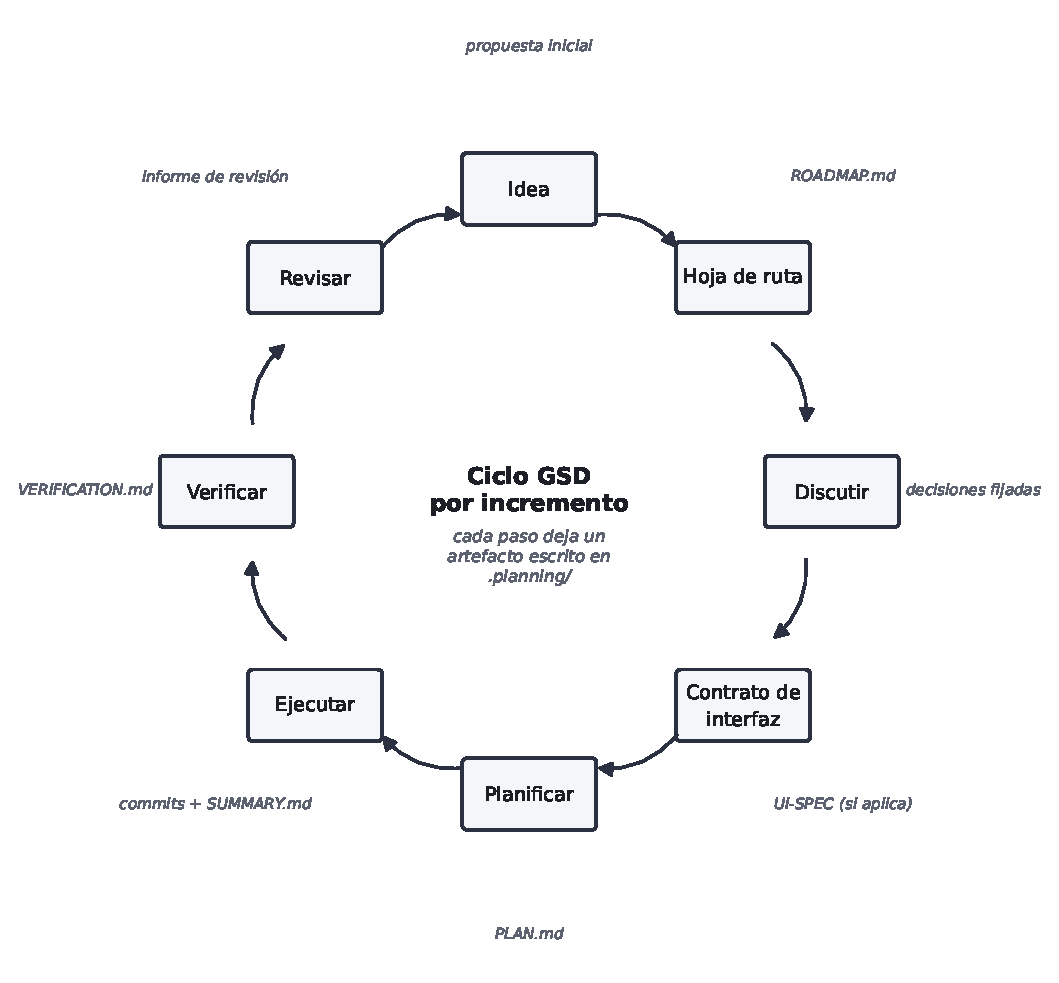
\includegraphics[width=0.72\textwidth]{figures/ciclo-gsd.pdf}
    \caption{Ciclo de un incremento en el método GSD y los artefactos que produce cada paso.}
    \label{fig:ciclo-gsd}
\end{figure}

En la práctica, cada incremento se abre con una discusión que fija por escrito sus decisiones
y supuestos. Si tiene interfaz, se establece además un contrato de diseño con sus componentes
y estados. A continuación se investiga y se redacta el plan, que lo descompone en tareas
atómicas con criterios de aceptación y se comprueba antes de tocar código. La ejecución
implementa ese plan, confirma los cambios en el control de versiones y registra en un resumen
lo realmente hecho y las desviaciones. Por último, la verificación comprueba, de forma
independiente, que el objetivo se ha alcanzado. Una revisión de código somete después los
cambios a un análisis de seguridad, rendimiento y corrección con un contexto distinto del que
los escribió. Cada incremento termina con una firma de aceptación del proyecto. Las órdenes de este flujo
(\texttt{discuss-phase}, \texttt{ui-phase}, \texttt{plan-phase}, \texttt{execute-phase},
\texttt{verify-work} y \texttt{code-review}), junto con \texttt{pause-work} y \texttt{resume-work} para
retomar el trabajo entre sesiones, se usaron de verdad durante el proyecto.

\section{Planificación viva y trazabilidad}\label{sec:met-planning}\label{sec:gestion-gsd}\label{sec:met-trazabilidad}\label{sec:met-incidencias}\label{sec:gestion-obsidian}

La cadena de artefactos que produce cada paso vive en el árbol \texttt{.planning/} del repositorio, que actúa como
la memoria de trabajo compartida entre el autor y los agentes. \texttt{PROJECT.md} recoge el
encuadre general del proyecto y las decisiones de producto que no cambian de una fase a otra.
\texttt{REQUIREMENTS.md} mantiene el catálogo de requisitos con su identificador, su estado y
la fase que lo cierra, de forma que un requisito se puede seguir desde que se declara hasta que
queda marcado como completo. \texttt{ROADMAP.md} descompone el proyecto en fases con sus planes
y su progreso. Las fases son las unidades de trabajo del \textit{roadmap}: están numeradas en
orden (con decimales, como la 01.1, cuando se insertó una posterior) y la memoria las cita por
ese número, por ejemplo la Fase~2 para el laboratorio de evaluación. \texttt{STATE.md} conserva un resumen del punto en el que se encuentra el
trabajo, con referencia al último commit relevante, pensado para que una sesión nueva, humana o
de agente, pueda retomar el hilo sin releer todo el historial. Cada fase añade además, dentro de
\texttt{.planning/phases/}, un par de documentos por plan: un \texttt{PLAN.md} que describe qué
se va a hacer y cómo se va a verificar y un \texttt{SUMMARY.md} que el agente ejecutor redacta
al terminar, con lo que se hizo, las desviaciones respecto al plan original y la evidencia que
lo respalda. Esta cadena de documentos es la que permite responder, meses después, a la
pregunta de por qué existe una línea de código concreta: se remonta al plan que la motivó, a la
verificación que la aceptó y al requisito que la justificaba, sin depender de la memoria de
nadie.

La Tabla~\ref{tab:planning-arbol} enumera los artefactos principales del árbol y su función.

\begin{table}[H]
\centering
\begin{tabularx}{\textwidth}{ | Y | Y | }
    \hline
    \textbf{Artefacto} & \textbf{Función} \\
    \hline
    \texttt{PROJECT.md} & Definición del producto, valor central, requisitos activos y fuera de alcance. \\
    \hline
    \texttt{REQUIREMENTS.md} & Catálogo de requisitos con identificador estable y matriz de trazabilidad a evidencia. \\
    \hline
    \texttt{ROADMAP.md} & Incrementos, objetivos, criterios de éxito y progreso. \\
    \hline
    \texttt{STATE.md} & Estado actual, posición, decisiones acumuladas y continuidad de sesión. \\
    \hline
    \path{phases/<incremento>/<plan>-PLAN.md} & Alcance y criterios de aceptación de un plan, antes de implementar. \\
    \hline
    \path{phases/<incremento>/<plan>-SUMMARY.md} & Lo realmente ejecutado, desviaciones y evidencias, al cerrar el plan. \\
    \hline
    \path{phases/<incremento>/<incremento>-VERIFICATION.md} & Verificación independiente del objetivo del incremento. \\
    \hline
    \path{phases/<incremento>/deferred-items.md} & Hallazgos fuera de alcance, enrutados a trabajo posterior. \\
    \hline
\end{tabularx}
\caption{Artefactos principales del árbol \texttt{.planning/}.}
\label{tab:planning-arbol}
\end{table}

La trazabilidad se apoya en tres mecanismos. El primero es la matriz de
\texttt{REQUIREMENTS.md}, que registra el estado de cada requisito y la evidencia que lo
cierra, de modo que cualquier requisito se puede seguir hasta el trabajo que lo entrega y
hasta la prueba que lo respalda. El segundo es la correspondencia entre planes e incidencias:
cada plan tiene una incidencia (\textit{issue}) abierta en el repositorio, que los mensajes de
commit referencian con \texttt{Refs \#N} mientras el plan avanza y que se cierra con
\texttt{Closes \#N} cuando el \texttt{SUMMARY.md} confirma que quedó ejecutado, integrado y
verificado. Así el historial de incidencias muestra, sin abrir el árbol \texttt{.planning/}, qué
trabajo está cerrado y con qué evidencia. El tercero es el registro
de agentes descrito en la Sección~\ref{sec:met-ledger}, que ata cada artefacto a la acción
que lo produjo mediante un hash de contenido. Entre los tres, una decisión de la memoria se
puede recorrer hacia atrás hasta su plan, su requisito y su discusión; hacia delante llega
hasta la prueba y la firma que la verifican.

Además del registro de agentes, el proyecto conserva dos registros de decisión. Los ítems
diferidos, en \texttt{deferred-items.md}, recogen los hallazgos fuera de alcance descubiertos
durante la ejecución, con su motivo y su destino. Los registros de decisión de arquitectura,
en \texttt{docs/adr/}, documentan cada decisión material con su contexto, sus alternativas,
su decisión, su evidencia, sus consecuencias y su reversibilidad. El
Capítulo~\ref{cap:diseno} resume los nueve registros de decisión de arquitectura vigentes.

El árbol \texttt{.planning/} es la fuente de verdad operativa, pero no está pensado para
explorar cómo se relacionan las ideas entre sí. Para eso, el proyecto mantiene además un
\textit{vault} de Obsidian, \texttt{ideas-vault/}, una colección de notas en Markdown
enlazadas entre sí mediante referencias internas que Obsidian representa como un grafo
navegable. Cada nota recoge un concepto (una decisión de diseño, un requisito, un algoritmo,
una fase); sus enlaces señalan de qué otras notas depende o a cuáles afecta, de modo que
retomar un concepto después de semanas sin tocarlo no exige reconstruir el contexto desde
cero: basta con abrir su nota y seguir sus enlaces. La Figura~\ref{fig:obsidian-vault} muestra
el grafo real del vault de SavePoint en el momento de escribir esta memoria, generado a partir
de los enlaces existentes entre sus notas, no como una ilustración esquemática.

\begin{figure}[H]
    \centering
    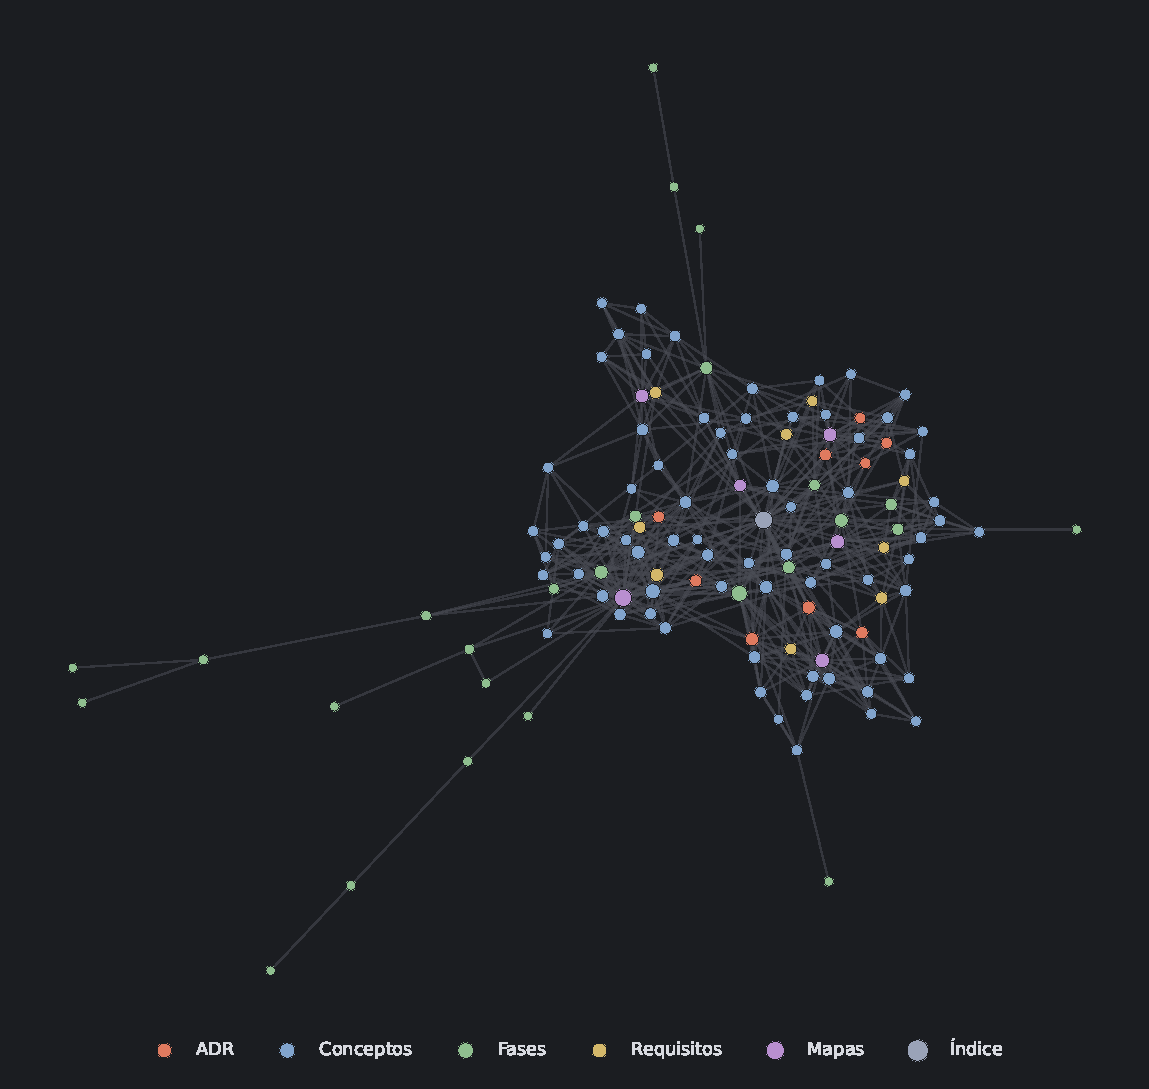
\includegraphics[width=0.92\textwidth]{figures/obsidian-vault-graph.pdf}
    \caption{Grafo del vault de Obsidian de SavePoint (\texttt{ideas-vault/}), coloreado por
    categoría de nota. Se muestra la componente conexa principal, ciento veintitrés notas de
    las ciento cincuenta que contiene el vault; el resto enlaza solo entre sí en subgrafos
    pequeños y aislados. Los nodos de mayor tamaño, como \texttt{00 - Indice} o los mapas de
    investigación y de datos, son las notas con más enlaces entrantes y salientes.}
    \label{fig:obsidian-vault}
\end{figure}

El vault y el árbol \texttt{.planning/} cumplen papeles distintos y deliberadamente no
redundantes. El árbol de planificación es normativo: fija alcance, criterios de aceptación y
evidencia; de él depende que un plan se dé o no por cerrado. El vault es descriptivo: enlaza
conceptos con las fuentes canónicas que los sustentan (un ADR, un requisito, una fase) para que
se puedan explorar sus relaciones de forma visual, pero nunca sustituye a las pruebas, a los
hashes ni a los artefactos versionados que certifican una decisión. Esta separación se aplicó
también a la propia redacción de esta memoria: antes de escribir varios de los capítulos que
siguen, resultó más rápido navegar el grafo del vault para recuperar cómo encajaban entre sí
conceptos ya explorados en sesiones distintas, semanas atrás, que releer el historial completo
de decisiones desde cero.

\section{Agentes especializados y contrato de contexto}\label{sec:met-agentes}\label{sec:met-subagentes}\label{sec:gestion-subagentes}\label{sec:gestion-worktrees}\label{sec:gestion-skills}\label{sec:met-contrato-contexto}\label{sec:gestion-contrato}\label{sec:gestion-memoria}\label{sec:met-ledger}\label{sec:gestion-ledger}\label{sec:met-convenciones}

El proyecto se desarrolló con asistencia sistemática de los agentes especializados que define
GSD. Conviene delimitar desde el principio el reparto de responsabilidades, que la
Sección~\ref{sec:met-encuadre} retoma: los agentes ejecutan, mientras que la definición del
alcance, los criterios de aceptación, la revisión de cada entrega y la decisión final son
del proyecto. El uso de agentes se describe aquí como una metodología de trabajo que se
diseñó, dirigió y evaluó, no como una coautoría.

El método de la Sección~\ref{sec:arte-agentes} se instrumenta en SavePoint con tres mecanismos.
El primero es el aislamiento del contexto: el trabajo se descompone en tareas atómicas, cada
una ejecutada por una instancia nueva del agente con la ventana limpia, y la información
viaja entre tareas por los ficheros persistentes del árbol \texttt{.planning/}
(Sección~\ref{sec:met-planning}), de modo que una interrupción, un límite de sesión o un
cambio de día no hacen perder el hilo. El segundo es la especialización de esas instancias en
los papeles de la Tabla~\ref{tab:subagentes}: quien planifica, quien implementa y quien
verifica son instancias independientes, de modo que la verificación no hereda la confianza
del código recién escrito, igual que en un equipo humano se separan el desarrollo y la
revisión.

\begin{table}[H]
\centering
\begin{tabularx}{\textwidth}{ | Y | Y | }
    \hline
    \textbf{Rol} & \textbf{Responsabilidad y límite} \\
    \hline
    \texttt{gsd-phase-researcher} & Recopila y sintetiza evidencia para planificar un incremento. Propone; etiqueta fuente, evidencia o supuesto. \\
    \hline
    \texttt{gsd-ui-researcher} / \texttt{gsd-ui-checker} & Convierten los requisitos en un contrato de diseño y lo validan. La comprobación automática de accesibilidad no sustituye la revisión humana. \\
    \hline
    \texttt{gsd-planner} & Divide el alcance en tareas verificables. Propone secuencia y gates; no declara terminado el producto. \\
    \hline
    \texttt{gsd-executor} & Implementa, prueba y registra correcciones en una copia de trabajo aislada, con commits atómicos. No se presenta como verificación independiente. \\
    \hline
    \texttt{gsd-verifier} & Verifica el objetivo del incremento de forma independiente y escribe el informe de verificación. \\
    \hline
    \texttt{gsd-code-reviewer} & Revisa todo el repositorio en busca de defectos con un contexto propio, distinto del de la implementación. \\
    \hline
\end{tabularx}
\caption{Subagentes empleados y su responsabilidad.}
\label{tab:subagentes}
\end{table}

El tercer mecanismo traslada ese aislamiento al sistema de ficheros mediante \textit{worktrees} de Git, copias de trabajo independientes que
comparten el mismo historial de repositorio pero permiten que varios agentes ejecutores avancen
en paralelo sin pisarse los cambios. El ciclo de un ejecutor es siempre el mismo: se crea un
\textit{worktree} nuevo para el plan que le corresponde, el agente trabaja y hace sus
\textit{commits} dentro de esa copia aislada, al terminar se integra el resultado en la rama
principal mediante una fusión sin avance rápido (\texttt{merge --no-ff}), que conserva visible
en el historial el conjunto de cambios de ese plan como una unidad; por último, se limpia el
\textit{worktree}. Cuando varios planes de una misma fase declaran el mismo requisito, la
orquestación añade además una comprobación de que todos esos planes tienen ya su
\texttt{SUMMARY.md} antes de marcar el requisito como cerrado, para que ningún requisito quede
completo mientras una de sus partes sigue pendiente en otro plan.

Además de los subagentes, el repositorio versiona \textit{skills}: procedimientos empaquetados
que un agente puede invocar para una tarea concreta y repetible, como revisar código con un
criterio fijo o preparar una entrega. Al vivir dentro del repositorio, junto al código que
producen, las \textit{skills} quedan sujetas al mismo control de versiones, a la misma revisión
y al mismo historial que cualquier otro artefacto del proyecto. El entorno de trabajo del
agente deja así de ser una configuración personal invisible para convertirse en parte del
entregable: cualquiera que clone el repositorio dispone del mismo procedimiento que se empleó
durante el desarrollo, no solo del resultado final.

Todo agente que empieza a trabajar en el repositorio, sea la herramienta que sea, lee primero
un conjunto fijo de ficheros de instrucciones que actúan como su contrato de contexto:
\texttt{AGENTS.md}, \texttt{CLAUDE.md} y \texttt{.github/copilot-instructions.md} declaran las
reglas que cualquier asistente debe seguir en este proyecto, mientras que
\texttt{CONVENTIONS.md} fija las convenciones concretas de idioma, de nomenclatura y de flujo de
trabajo con incidencias. Un ejemplo transversal de regla en ese contrato es la convención de
idioma del proyecto: la documentación de este TFG se escribe en español, el código y sus
comentarios se escriben en inglés. Esa regla se aplica sin excepción con independencia de qué
herramienta esté trabajando en cada momento, precisamente porque vive en un fichero que todas
ellas leen al empezar, en lugar de depender de que alguien la recuerde y la repita en cada
conversación.

Sobre ese mismo contrato se apoyan los ficheros de memoria del agente, que sobreviven entre
sesiones: cuando un error del agente o una corrección del proyecto tiene valor general, se
destila en una regla que se relee al iniciar cada tarea, de modo que el fallo no se repite. El
proyecto acumuló varias reglas de este tipo a partir de incidencias reales:

\begin{itemize}
    \item La lista de identificadores de Wikidata escrita a mano en el guion de adquisición
    contenía entidades que no eran videojuegos. La regla derivada obliga a verificar en vivo
    cualquier identificador de Wikidata antes de usarlo, sin confiar en la memoria ni en un
    commit anterior.
    \item El primer intento de cargar el catálogo de IGDB junto al corpus de Wikidata abortó
    por una colisión de \textit{slug} de plataforma. La corrección enseñó al importador a
    reconciliar una plataforma existente por \textit{slug}, nombre e inserción dentro de un
    savepoint, en lugar de fallar.
    \item Los enganches de GSD fallaban en Windows por un problema de shell. Detectarlo y
    corregirlo pronto evitó que el resto del trabajo tropezara con lo mismo.
    \item Sin un montaje enlazado de Docker y sin cargar el módulo de configuración de Django
    dentro del contenedor, toda verificación posterior habría probado una imagen obsoleta o
    habría fallado al arrancar. Corregir ambos al detectarlos evitó que el trabajo siguiente
    chocara con la misma pared.
\end{itemize}

El componente más distintivo del proceso es el registro de agentes,
\texttt{docs/methodology/agent-ledger.jsonl}, un fichero de solo anexado con un objeto por
línea. Cada entrada lleva una marca de tiempo, un tipo, el actor, el objetivo, las entradas y
salidas referenciadas por ruta relativa y hash SHA-256, las herramientas empleadas sin sus
secretos, el resultado y las limitaciones declaradas. El tipo es uno de tres:
\texttt{proposal} para una propuesta de agente, \texttt{automated-check} para una
comprobación determinista y \texttt{author-decision} para una decisión humana, que siempre
identifica al actor como persona. El registro contiene veinticinco entradas. El gate
\texttt{scripts/check-evidence.ps1} valida su esquema, sus tipos, sus actores, sus rutas, sus
hashes y su cobertura, probando primero con entradas inválidas antes de dar por buena una
ejecución limpia.

El registro es una convención auditable, no un almacén criptográficamente inmutable: Git
conserva las revisiones y el gate detecta corrupción de referencias en el estado actual, pero
un actor con permiso de escritura podría reescribir el historial. Para la evidencia final se
firma o etiqueta el commit correspondiente. El registro es honesto sobre sus propios huecos:
donde un artefacto histórico resultó irrecuperable, la entrada lo declara en sus campos de
entradas no verificables y de limitaciones en lugar de ocultarlo o falsearlo. También registra
que el proyecto usó más de un entorno de agente, con modelos distintos en el
trabajo inicial y en el posterior, con la advertencia de que un nombre de
modelo no basta para reproducir una salida probabilística: la evidencia reproducible son los
artefactos versionados, los hashes, los comandos y las decisiones humanas.

Los mensajes de commit siguen el estilo de \textit{Conventional Commits} y se escriben en
inglés. 

\section{Planificación del laboratorio de evaluación}\label{sec:met-fase2}

La Fase 2 se planificó como el puente entre la demostración de producto y la evaluación
reproducible. Su objetivo no era añadir una pantalla aislada, sino fijar las condiciones que
permiten afirmar algo sobre un recomendador: qué obras entran en el corpus, qué significan
las valoraciones, qué usuarios se simulan, cómo se construyen los candidatos y con qué
métricas se comparan las listas. Las decisiones metodológicas se tomaron antes de cualquier
ejecución de laboratorio y se conservaron en el directorio de planes de la fase.

El orden no es accidental. El corpus y el snapshot preceden al protocolo; el protocolo
precede a la generación de usuarios y a la implementación de variantes; y solo entonces se
puede ejecutar una comparación con garantías de que todos los algoritmos han recibido la
misma partición y el mismo conjunto de candidatos. Una tarea completada ha superado las
verificaciones de su contrato, pero no demuestra una superioridad algorítmica.

Las decisiones que bloquean una comparación posterior quedaron congeladas en
\texttt{docs/methodology/protocol.json} y en \texttt{docs/methodology/evaluation-protocol.md}:
el corpus, el significado de las valoraciones, la población sintética, la relevancia, el
conjunto de candidatas y las métricas. Esta sección solo recoge cómo se planificó esa
congelación; el contenido de cada decisión se describe donde se aplica. El corpus y los
ratings, en la Sección~\ref{cap:datos}; el diseño del laboratorio, en la
Sección~\ref{sec:dis-laboratorio}; y el protocolo con el que se publicaron los resultados, en
la Sección~\ref{sec:exp-protocolo}.

\section{Planificación temporal}\label{sec:met-temporal}

El trabajo se planificó como una sucesión de incrementos verticales, cada uno utilizable y
verificado antes de abordar el siguiente, en lugar de un calendario cerrado de tareas fijado
desde el principio. El desarrollo se organizó en seis iteraciones a lo largo de cuatro meses,
del 2 de junio al 30 de septiembre de 2026, agrupadas alrededor de los hitos de la
Tabla~\ref{tab:hitos}.

\begin{table}[H]
\centering
\caption{Lista de hitos del trabajo.}\label{tab:hitos}
\begin{tabularx}{\textwidth}{ | Y | Y | }
    \hline
    \textbf{Hito} & \textbf{Fecha} \\
    \hline
    H0 — Aprobación de la propuesta y arranque del repositorio & 02/06/2026 \\
    \hline
    H1 — Demostración pública de tres días en producción (Fase 1) & 12/06/2026 \\
    \hline
    H2 — Catálogo a escala real e interfaz rediseñada (Fase 01.1) & 03/07/2026 \\
    \hline
    H3 — Contrato de evaluación offline congelado (Fase 2) & 24/07/2026 \\
    \hline
    H4 — Recomendadores de contenido, colaborativo e híbrido implementados & 14/08/2026 \\
    \hline
    H5 — Publicación de resultados v15 con significación estadística & 12/09/2026 \\
    \hline
    H6 — Flujos de colección, relaciones de amistad y endurecimiento cerrados & 14/09/2026 \\
    \hline
    H7 — Memoria del TFG completa, lista para defensa & 30/09/2026 \\
    \hline
\end{tabularx}
\end{table}

La Figura~\ref{fig:calendario} sitúa las iteraciones y los hitos en el calendario.

\begin{figure}[htp]
    \centering
    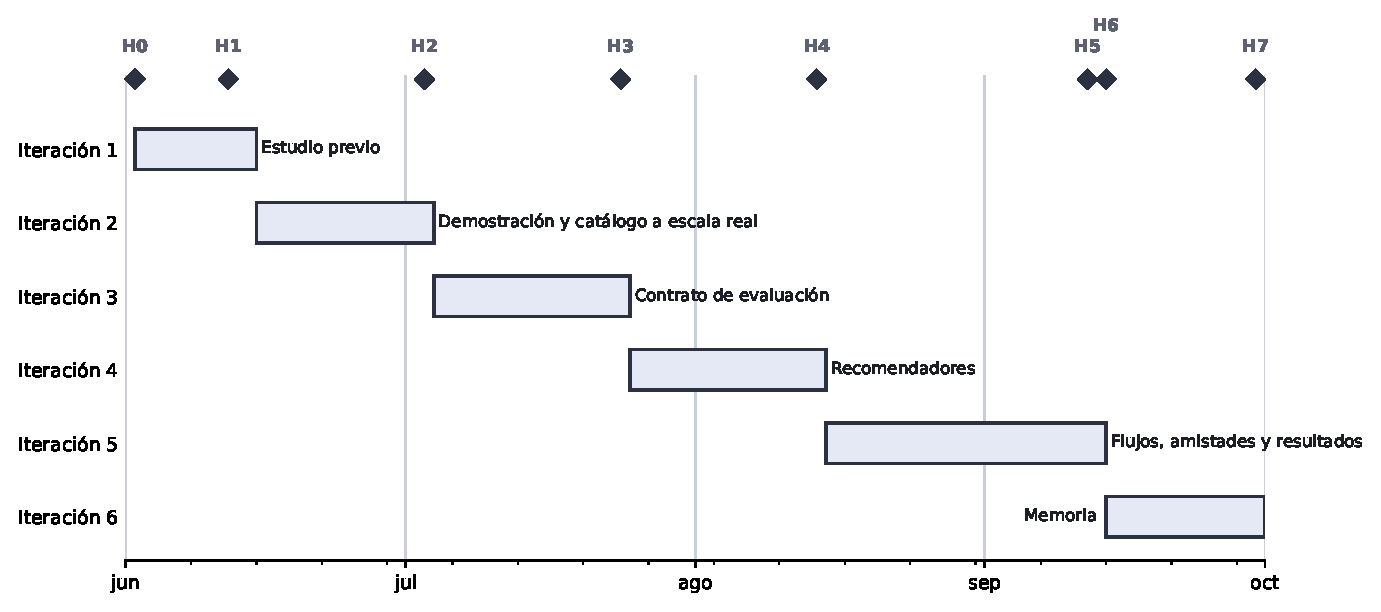
\includegraphics[width=0.9\textwidth]{figures/calendario-iteraciones.pdf}
    \caption{Calendario de las iteraciones y de los hitos H0 a H7 del trabajo.}
    \label{fig:calendario}
\end{figure}

La \textbf{Iteración 1} (2 al 14 de junio) cubrió el estudio previo: revisión de productos de
referencia, comparación de fuentes de datos de videojuegos y sus licencias, y las primeras
decisiones de arquitectura (ADR-001 y ADR-002); cerró con un entorno de desarrollo
reproducible en Docker Compose. La \textbf{Iteración 2} (15 de junio al 3 de julio) entregó el
primer incremento de producto bajo una restricción explícita de tres días para una
demostración pública visible, con un catálogo reducido, una cuenta y la recomendación por
popularidad; a continuación amplió el catálogo a escala real e incorporó el rediseño de la
interfaz. La \textbf{Iteración 3} (4 al 24 de julio) congeló el contrato de evaluación offline:
corpus, población sintética, métricas y protocolo, antes de escribir ningún algoritmo de
recomendación avanzado. La \textbf{Iteración 4} (25 de julio al 14 de agosto) implementó las
tres familias de recomendación (contenido, colaborativo e híbrido) y sus dieciséis variantes.
La \textbf{Iteración 5} (15 de agosto al 13 de septiembre) cerró los flujos completos de
colección y portabilidad, las relaciones de amistad y el endurecimiento de seguridad; ejecutó también la publicación final de resultados (v15) descrita en el
Capítulo~\ref{cap:resultados}. La \textbf{Iteración 6} (14 al 30 de septiembre) se dedicó por
completo a la redacción, revisión y cierre de esta memoria.

\section{Estimación de esfuerzo y presupuesto}\label{sec:met-presupuesto}

El proyecto no llevó un registro de horas minuto a minuto por tarea, de modo que la estimación
de esfuerzo que sigue se reconstruye a partir de la duración de cada iteración y de la carga de
trabajo declarada de un estudiante que compagina el TFG con otras obligaciones académicas,
en torno a veinticinco horas semanales durante las diecisiete semanas del proyecto. Tomando
como unidad el bloque de trabajo, no el incremento, la Tabla~\ref{tab:presupuesto-horas}
reparte esas horas entre las grandes áreas del trabajo.

\begin{table}[H]
\centering
\caption{Estimación de horas por bloque de trabajo.}\label{tab:presupuesto-horas}
\begin{tabularx}{\textwidth}{ | Y | Z | }
    \hline
    \textbf{Bloque} & \textbf{Horas estimadas} \\
    \hline
    Análisis, requisitos y diseño & 60 \\
    \hline
    Infraestructura reproducible y despliegue & 35 \\
    \hline
    Implementación de producto (backend y frontend) & 120 \\
    \hline
    Adquisición y gobierno de datos & 40 \\
    \hline
    Algoritmos de recomendación y protocolo de evaluación & 90 \\
    \hline
    Pruebas, verificación y revisión & 45 \\
    \hline
    Redacción de la memoria & 50 \\
    \hline
    \textbf{Total} & \textbf{440} \\
    \hline
\end{tabularx}
\end{table}

El coste directo se calcula sobre esas 440 horas con una tarifa de referencia de un perfil
junior de ingeniería del software en España, 14,00\,€/hora, una cota conservadora frente al
coste real de contratación de un perfil equivalente. El coste material recoge la amortización
proporcional del equipo personal empleado (un portátil de gama media, con una vida útil
estimada de cuatro años, del que este trabajo consume cuatro meses); no se incluye ningún coste
de infraestructura en la nube, porque la topología de despliegue público se diseñó
explícitamente de coste cero (ADR-005, Sección~\ref{cap:despliegue}). El coste indirecto
recoge la cuota proporcional de cuatro meses de electricidad y conexión a internet atribuible
al proyecto. La Tabla~\ref{tab:presupuesto} resume el presupuesto total.

\begin{table}[H]
\centering
\begin{tabularx}{\textwidth}{ | Y | Z | }
    \hline
    \textbf{Concepto} & \textbf{Coste (\euro{})} \\
    \hline
    Coste directo (440\,h a 14,00\,€/h) & 6.160,00 \\
    \hline
    Coste material (amortización de equipo, 4 meses) & 75,00 \\
    \hline
    Costes indirectos (electricidad y conexión, 4 meses) & 180,00 \\
    \hline
    \textbf{Presupuesto total} & \textbf{6.415,00} \\
    \hline
\end{tabularx}
\caption{Estimación de esfuerzo y presupuesto del proyecto.}
\label{tab:presupuesto}
\end{table}

Estas cifras son una estimación reconstruida a posteriori, no una medición registrada durante
el desarrollo; así debe entenderse cualquier comparación futura entre coste estimado y coste
real.

\section{Riesgos y mitigaciones}\label{sec:met-riesgos}

La Tabla~\ref{tab:riesgos} recoge los riesgos que se identificaron y cómo se mitigaron o se
mantienen bajo vigilancia.

\begin{table}[H]
\centering
\begin{tabularx}{\textwidth}{ | Y | Y | }
    \hline
    \textbf{Riesgo} & \textbf{Mitigación} \\
    \hline
    Restricción de tres días del primer incremento público & Alcance de demostración deliberadamente estrecho: catálogo pequeño, una cuenta y recomendación por popularidad. \\
    \hline
    Términos legales de las fuentes de datos & Confirmación caso por caso: corpus de Wikidata bajo dominio público, términos de IGDB registrados textualmente y reconciliados en un registro de decisión. \\
    \hline
    Volumen de IGDB en una importación larga & Importador reanudable por cursor de identificador, con checkpoint tras cada lote y resistencia probada a una interrupción. \\
    \hline
    Portadas por enlace directo a un tercero & Ventana de retención de treinta días asumida; ausencia o fallo de una portada cae a un marcador propio. \\
    \hline
    El protocolo de evaluación debe congelarse antes de comparar recomendadores & El heurístico de géneros del sistema se declaró explícitamente fuera de esa comparación desde el principio; la comparación en sí se congeló y se ejecutó más tarde, como recoge el Capítulo~\ref{cap:resultados}. \\
    \hline
    Errores del agente en trabajo dado por bueno & Verificación de objetivos independiente y revisión de código de todo el repositorio con contexto propio. \\
    \hline
    Despliegue no conectado a datos reales & Decisión registrada del proyecto de posponer esa conexión al final del proyecto; el entorno local reproducible es la vía de demostración. \\
    \hline
\end{tabularx}
\caption{Riesgos identificados y sus mitigaciones.}
\label{tab:riesgos}
\end{table}

\section{Lecciones aprendidas y valoración de la metodología}\label{sec:met-desviaciones}\label{sec:met-encuadre}\label{sec:gestion-beneficios}\label{sec:gestion-limitaciones}

El trabajo dejó varias lecciones de ingeniería que conviene recoger. La primera tiene que ver
con el despliegue. La topología pasó de un único proveedor con
predespliegue para las dos imágenes de contenedor a tres servicios gratuitos coordinados, al
chocar la restricción de coste cero con el modelo de un solo proveedor. La decisión y sus
consecuencias quedaron documentadas en un registro de decisión de arquitectura, de modo que
la diferencia entre el despliegue público y el entorno local es una elección deliberada y
no una divergencia de comportamiento.

La segunda es de higiene del propio proceso: un gate de evidencia llegó a estar en rojo en la
rama principal por un problema de fin de línea y por registros de decisión escritos en inglés
antes de fijarse la convención de idioma. Corregirlo en cuanto se detectó evitó que el resto
del trabajo arrastrara un gate poco fiable. Estas incidencias, junto con otras menores,
quedaron registradas en los resúmenes de plan.

El enfoque produjo beneficios concretos y observables en el proyecto, junto con límites que
conviene declarar con la misma franqueza. El alcance se mantuvo bajo control a lo largo de
sucesivos incrementos, sin que el trabajo de uno se filtrara en otro, y cada cambio quedó
trazado hasta su plan, su requisito y su evidencia. Las revisiones de código con contexto
independiente encontraron dieciséis hallazgos reales, descritos en la
Sección~\ref{cap:pruebas}, que se corrigieron por completo, incluidos defectos de seguridad en
trabajo ya dado por bueno. El trabajo se pudo reanudar sin pérdida de hilo tras interrupciones
y límites de sesión, porque el estado vivía en ficheros y no en una conversación, y el propio
proceso de ingeniería quedó reproducible, no solo el producto: un tercero puede clonar el
repositorio y reconstruir la historia de decisiones a partir del árbol de planificación, los
registros de decisión, el registro de agentes y los gates de evidencia.

El enfoque depende, sin embargo, de la calidad de la especificación escrita: un plan ambiguo
produce una ejecución ambigua. Mantener la disciplina de planificación, verificación y registro
tiene un coste de tiempo notable para un TFG individual, y los agentes cometieron errores que
hubo que detectar y corregir, algunos de ellos recogidos en la
Sección~\ref{sec:met-contrato-contexto}. Un agente no es un evaluador independiente de su
propia propuesta, del mismo modo que un hash prueba identidad de bytes, no veracidad ni calidad;
por eso el enfoque no sustituye el juicio del proyecto sobre arquitectura, alcance y aceptación,
sino que lo enmarca. Existe un informe de uso de herramientas de asistencia, independiente y
posterior, que cubre la transparencia de su empleo; esta memoria ni lo suple ni lo contradice.

Los capítulos siguientes aplican ese método al análisis, al diseño y a la construcción del sistema.
